\documentclass[10pt, compress]{beamer}

\usepackage{listings}

\lstset{
  language = Prolog,
  basicstyle = \scriptsize \ttfamily,
  numbers = left,
  numberstyle = \tiny
}

\usetheme{m}
%\usepackage[utf8]{inputenc}
%\usepackage[T1]{fontenc}
\usepackage[document]{ragged2e} %Incluido por DHE
\usepackage{caption} %Incluido por DHE
\usepackage{subcaption} %Incluido por DHE
\usepackage{amsmath}
\usepackage{booktabs}
\usepackage[scale=2]{ccicons}
\usepackage{minted}
\usepackage{xcolor}
\usepackage{comment}
\usemintedstyle{trac}
\usepackage[english,spanish]{babel}
\selectlanguage{spanish}
\DeclareMathOperator*{\argmax}{argmax}

\usepackage{multirow}


\title{Cómputo Evolutivo}
\subtitle{Proyecto Final}
\date{26 junio 2019}
\author{\textbf{Arturo Márquez Flores}}
\institute{
\url{https://github.com/arturomf94/PSO}}
\begin{document}

\maketitle

\begin{frame}[fragile]
  \frametitle{Contenido}
  
  \begin{itemize}
      \item Introducción \\
      \item Bibliografía\\
      \item Teoría\\
      \item Evaluación y Resultados\\ 
      \item Conclusiones
  \end{itemize}

\end{frame}

\section{Introducción}

\begin{frame}[fragile]
  \frametitle{Relevancia}
    \begin{center}
        \textbf{La topología de comunicación impacta la tasa de convergencia.} 
    \end{center}{}
\end{frame}

\begin{frame}[fragile]
  \frametitle{Relevancia}
    \begin{center}
        \textbf{La mayoría de la literatura en PSO se enfoca en problemas sin restricciones.} 
    \end{center}{}
\end{frame}

\begin{frame}[fragile]
  \frametitle{Relevancia}
    \begin{center}
        \textbf{La literatura que estudia el impacto de la topología en problemas con restricciones es escaza.} 
    \end{center}{}
\end{frame}


\section{Bibliografía}

\begin{frame}[fragile]
  \frametitle{Primer PSO}
    \begin{center}
        Primer modelo en (Kennedy \& Eberhart, 1995, \cite{kennedy95}). 
    \end{center}{}
\end{frame}

\begin{frame}[fragile]
  \frametitle{Topologías}
    \begin{center}
        Primer estudio sobre el impacto de la topología en (Kennedy, 1999, \cite{kennedy99}). 
    \end{center}{}
\end{frame}

\begin{frame}[fragile]
  \frametitle{Restricciones}
    \begin{center}
        Uno de los primeros estudios sobre PSO con restricciones en  (Parsapoulos \& Vrahatis, 2002, \cite{parsopoulos02}). 
    \end{center}{}
\end{frame}

\begin{frame}[fragile]
  \frametitle{Topologías Dinámicas}
    \begin{center}
        Existen varios estudios sobre topologías dinámicas, como \cite{clerc06}, \cite{suganthan99}, \cite{marinakis13} y \cite{lim14}. 
    \end{center}{}
\end{frame}

\begin{frame}[fragile]
  \frametitle{Topologías Dinámicas y  Restricciones}
    \begin{center}
        Topologías dinámicas + Restricciones (\cite{bonyadi14} + \cite{bonyadi14_2}) 
    \end{center}{}
\end{frame}

\section{Teoría}

\begin{frame}[fragile]
  \frametitle{PSO Original}
    \begin{center}
         $v_{t + 1}^i = \omega v_t^i + \phi_1 R_{1,t}^i(p_t^i- x_t^i) + \phi_2 R_{2,t}^i(g_t^i- x_t^i) $
    \end{center}{}
\end{frame}

\begin{frame}[fragile]
  \frametitle{Global Best}
    \begin{center}
         $g_t^i = \argmax_{p_{t}^j \in P_t}  \{f(p_{t}^j): j \in N_t^i\}$
    \end{center}{}
\end{frame}

\begin{frame}[fragile]
  \frametitle{PSO}
    \begin{center}
    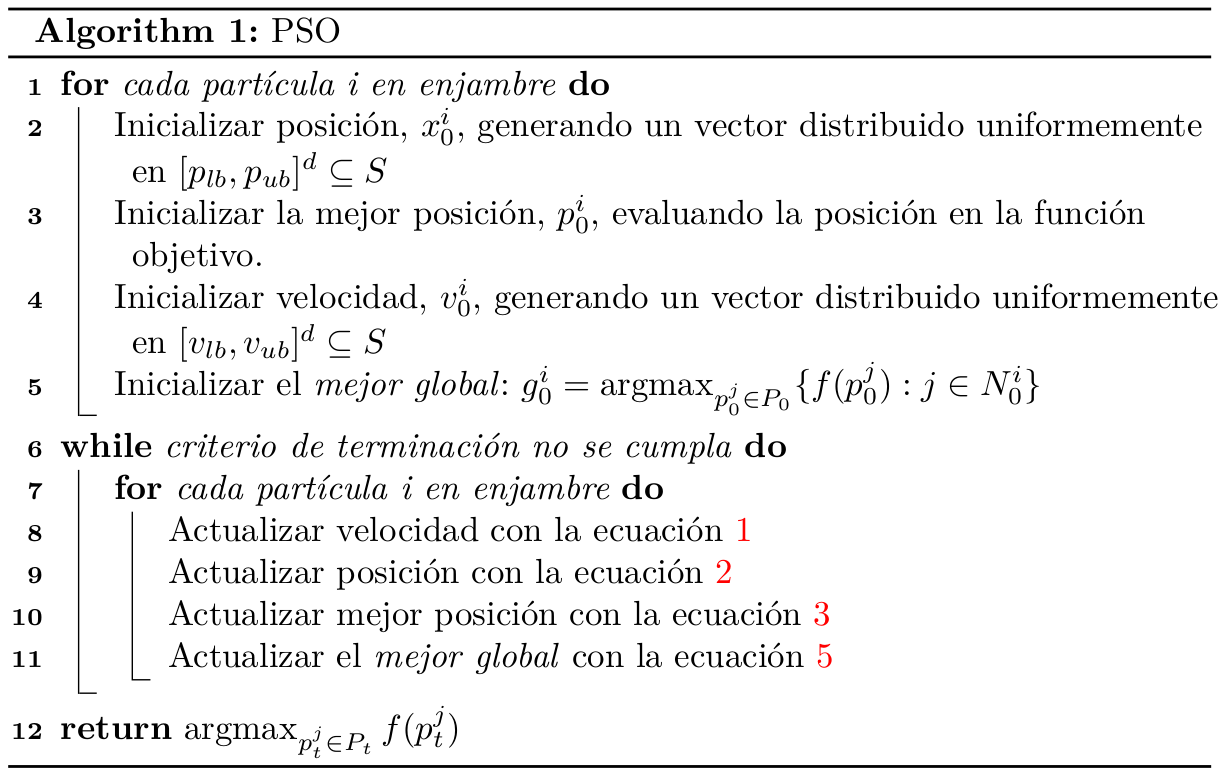
\includegraphics[scale=0.2]{pso.png}
    \end{center}
\end{frame}

\begin{frame}[fragile]
  \frametitle{Propuesta}
    \begin{center}
        \begin{itemize}
            \item Propuesta 1: sólo considerar posiciones factibles, siguiendo a \cite{xiahoui02}.
            \item Propuesta 2: modificar la topología aumentando el grado de los nodos, siguiendo a \cite{suganthan99}.
        \end{itemize}{}
    \end{center}{}
\end{frame}

\begin{frame}[fragile]
  \frametitle{Propuesta}
    \begin{center}
        \begin{itemize}
            \item $v_{t + 1}^i = \omega v_t^i + \phi_1 R_{1,t}^i(p_t^i- x_t^i) + \phi_2 R_{2,t}^i(g_t^i- x_t^i)$
            \item $v_{t + 1}^i = \omega v_t^i + \phi_2 R_{2,t}^i(g_t^i- x_t^i)$
        \item $v_{t + 1}^i = \omega v_t^i +  r_t^i$
        \end{itemize}{}
    \end{center}{}
\end{frame}

\begin{frame}[fragile]
  \frametitle{PSO Modificado}
    \begin{center}
    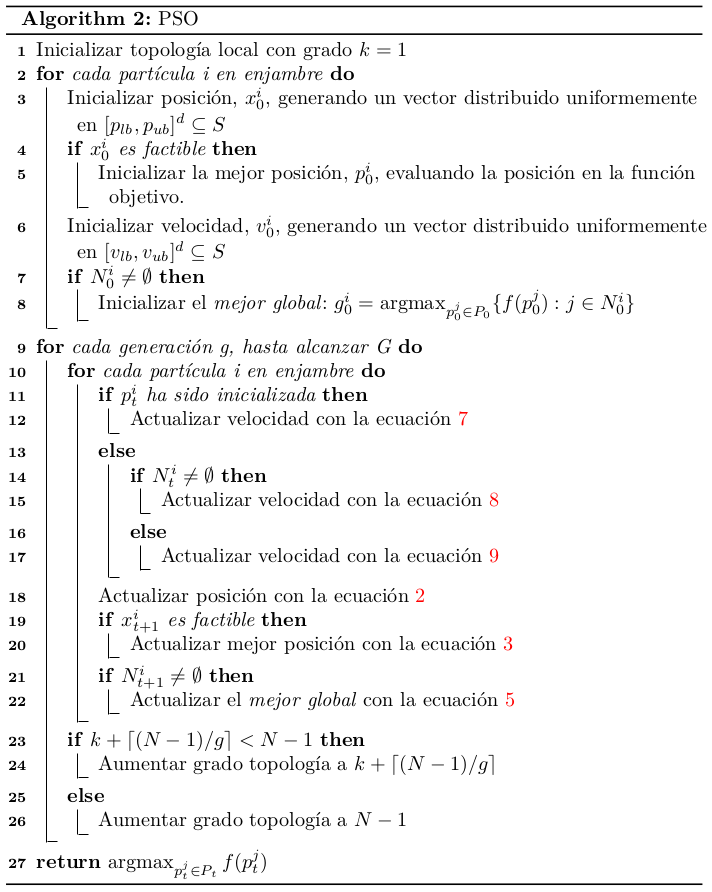
\includegraphics[scale=0.25]{mpso.png}
    \end{center}
\end{frame}

\section{Evaluación y Resultados}

\begin{frame}[fragile]
  \frametitle{Diseño}
    \begin{center}
         Se utilizará el benchmark del \href{http://web.mysites.ntu.edu.sg/epnsugan/PublicSite/Shared%20Documents/CEC-2017/Constrained/Technical%20Report%20-%20CEC2017-%20Final.pdf}{\textbf{reporte técnico}} en \cite{suganthan16}
    \end{center}{}
\end{frame}

\begin{frame}[fragile]
  \frametitle{Benchmark}
    \begin{center}
         \begin{itemize}
             \item 28 COPs
             \item Dimensiones 10, 30, 50 y 100.
             \item 2000D, 10000D y 20000D evaluaciones en la función objetivo.
             \item 25 corridas
             \item Número de violaciones a las restricciones para diferentes grados de tolerancia (1, 0.01 y 0.0001).
             \item Tasa de factibilidad y la comlpejidad del algoritmo
         \end{itemize}{}
    \end{center}{}
\end{frame}

\begin{frame}[fragile]
  \frametitle{Resultados Preliminares }
    \begin{center}
         \begin{itemize}
             \item C01, C03, C04, C06, C07, C11, C13 y C19
             \item Dimensiones 10 y 30. 
             \item Límites de evaluaciones en la función objetivo en 2,000, 10,000 y 20,000
         \end{itemize}{}
    \end{center}{}
\end{frame}

\begin{frame}[fragile]
  \frametitle{Resultados Preliminares}
    \begin{center}
         \begin{itemize}
             \item 200 partículas. 
             \item 100 iteraciones. 
             \item $c_1 = 0.6$, $c_2 = 0.3$ y $w = 0.4$.
         \end{itemize}{}
    \end{center}{}
\end{frame}

\begin{frame}[fragile]
  \frametitle{Resultados Preliminares}
    \begin{center}
         \begin{itemize}
             \item Los resultados pueden replicarse en \href{https://colab.research.google.com/github/arturomf94/PSO/blob/master/DTPSOCOP.ipynb}{\textbf{este colab}} 
             \item la librería utilizada se encuentra en \href{https://github.com/arturomf94/pyswarms}{\textbf{este repositorio}}
         \end{itemize}{}
    \end{center}{}
\end{frame}

\begin{frame}[fragile]
  \frametitle{Resultados Preliminares}
    \begin{center}
         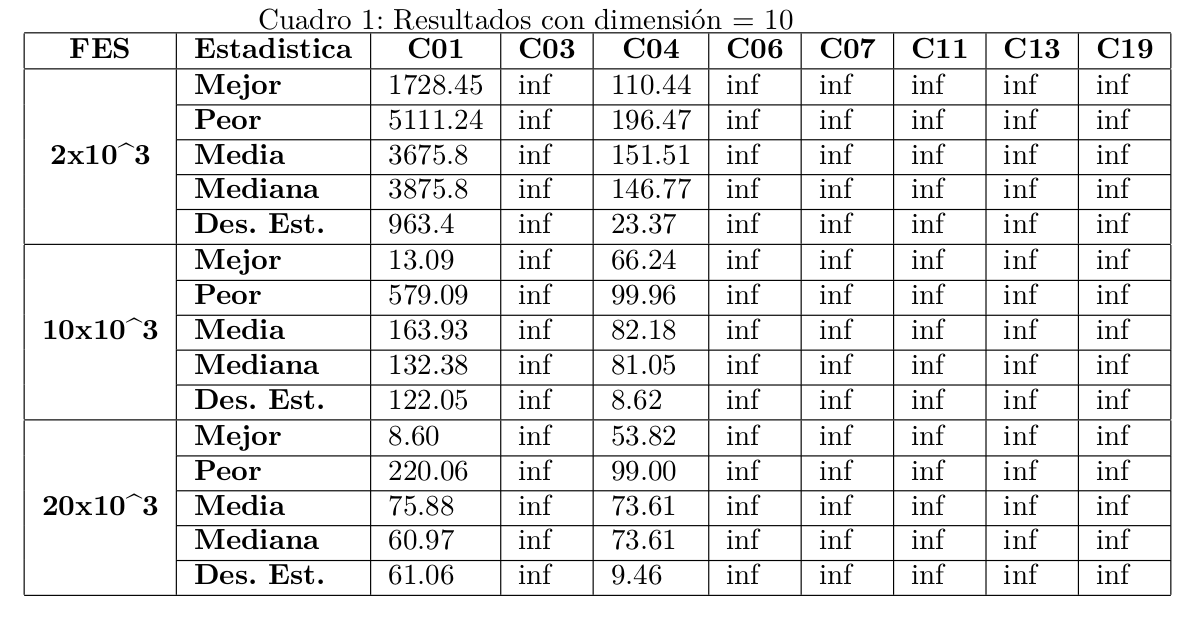
\includegraphics[scale=0.25]{10dim.png}
    \end{center}{}
\end{frame}

\begin{frame}[fragile]
  \frametitle{Resultados Preliminares}
    \begin{center}
         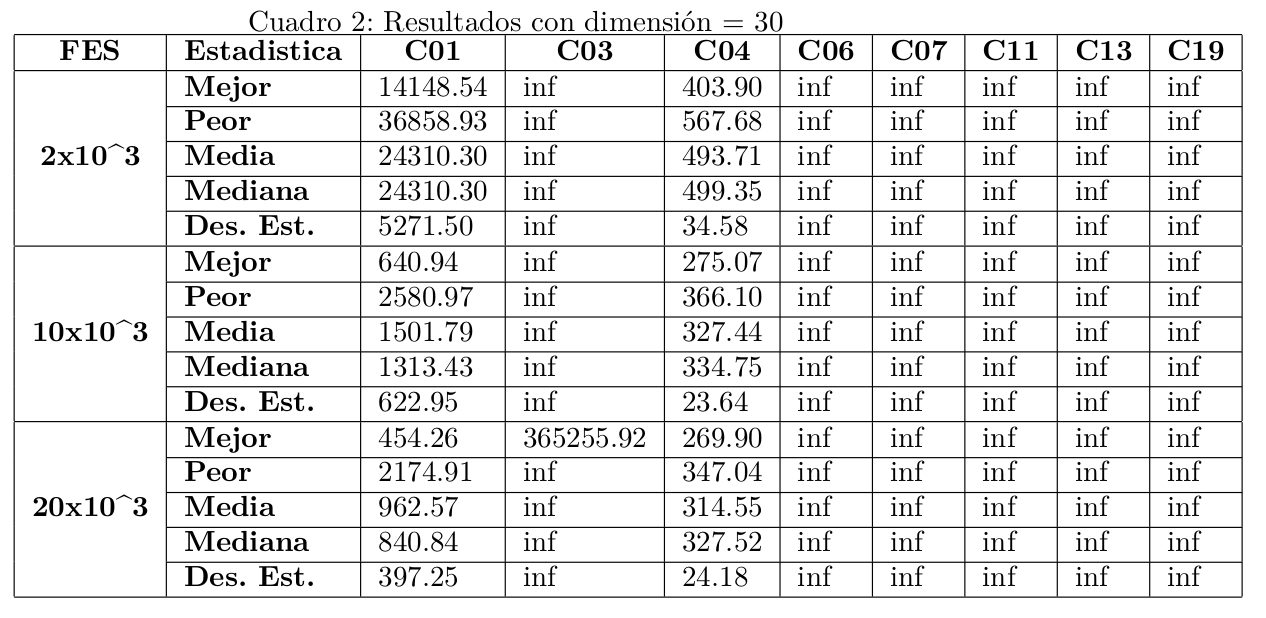
\includegraphics[scale=0.25]{30dim.png}
    \end{center}{}
\end{frame}

\section{Conclusiones}

\begin{frame}[fragile]
  \frametitle{Comentarios}
    \begin{center}
         Algoritmo no sirve para restricciones de igualdad.
    \end{center}{}
\end{frame}

\begin{frame}[fragile]
  \frametitle{Comentarios}
    \begin{center}
         Algoritmo no sirve para restricciones de desigualdad complejos.
    \end{center}{}
\end{frame}

\begin{frame}[fragile]
  \frametitle{Comentarios}
    \begin{center}
         Algoritmo no es competitivo en restricciones de desigualdad (en general).
    \end{center}{}
\end{frame}

\begin{frame}[fragile]
  \frametitle{Mejoras}
    \begin{center}
         El último punto puede arreglarse encontrando mejores parámetros y mejorando los límites del experimento.
    \end{center}{}
\end{frame}

\begin{frame}[fragile]
  \frametitle{Mejoras}
    \begin{center}
         Los primeros dos puntos podrían atacarse si primero se buscan las regiones factibles mediante la minimización del valor absoluto de las restricciones, tanto de igualdad como de desigualdad.
    \end{center}{}
\end{frame}

\bibliographystyle{alpha}
\bibliography{refs} 

\end{document}